\documentclass[12pt,a4paper]{article}
\usepackage{amsmath,amscd,amsbsy,amssymb,latexsym,url,bm,amsthm}
\usepackage{epsfig,graphicx,subfigure}
\usepackage{enumitem,balance}
\usepackage{wrapfig}
\usepackage{mathrsfs,euscript}
\usepackage[usenames]{xcolor}
\usepackage{hyperref}
\usepackage[vlined,ruled,linesnumbered]{algorithm2e}
\usepackage{amsmath}
\usepackage{booktabs}
\usepackage{threeparttable}
\usepackage{graphicx} %插入图片的宏包
\usepackage{float} %设置图片浮动位置的宏包
\usepackage{subfigure} %插入多图时用子图显示的宏包
\usepackage{listings}
\usepackage{natbib}
\usepackage{amssymb,amsmath}
\usepackage{color}
\hypersetup{colorlinks=true,linkcolor=black}

\newtheorem{theorem}{Theorem}
\newtheorem{lemma}[theorem]{Lemma}
\newtheorem{proposition}[theorem]{Proposition}
\newtheorem{corollary}[theorem]{Corollary}
\newtheorem{exercise}{Exercise}
\newtheorem*{solution}{Solution}
\newtheorem{definition}{Definition}
\theoremstyle{definition}

\renewcommand{\thefootnote}{\fnsymbol{footnote}}

\newcommand{\postscript}[2]
{\setlength{\epsfxsize}{#2\hsize}
	\centerline{\epsfbox{#1}}}

\renewcommand{\baselinestretch}{1.0}

\setlength{\oddsidemargin}{-0.365in}
\setlength{\evensidemargin}{-0.365in}
\setlength{\topmargin}{-0.3in}
\setlength{\headheight}{0in}
\setlength{\headsep}{0in}
\setlength{\textheight}{10.1in}
\setlength{\textwidth}{7in}
\makeatletter \renewenvironment{proof}[1][Proof] {\par\pushQED{\qed}\normalfont\topsep6\p@\@plus6\p@\relax\trivlist\item[\hskip\labelsep\bfseries#1\@addpunct{.}]\ignorespaces}{\popQED\endtrivlist\@endpefalse} \makeatother
\makeatletter
\renewenvironment{solution}[1][Solution] {\par\pushQED{\qed}\normalfont\topsep6\p@\@plus6\p@\relax\trivlist\item[\hskip\labelsep\bfseries#1\@addpunct{.}]\ignorespaces}{\popQED\endtrivlist\@endpefalse} \makeatother

\begin{document}
	\noindent
	
	%========================================================================
	\noindent\framebox[\linewidth]{\shortstack[c]{
			\Large{\textbf{Lab05-DynamicProgramming}}\vspace{1mm}\\
			CS214-Algorithm and Complexity, Xiaofeng Gao, Spring 2021.}}
	\begin{center}
		\footnotesize{\color{red}$*$ If there is any problem, please contact TA Haolin Zhou.}
		
		% Please write down your name, student id and email.
		\footnotesize{\color{blue}$*$ Name:Zirui Liu  \quad Student ID:519021910343 \quad Email: L.Prime@sjtu.edu.cn}
		
	\end{center}
	
	\begin{enumerate}
		\item \textit{Optimal Binary Search Tree.} Given a sorted sequence $K=\left \langle k_{1}, k_{2}, \ldots, k_{n} \right \rangle$ of $n$ distinct keys, and we wish to build a binary search tree from these keys. For each key $k_{i}$, we have a probability $p_{i}$ that a search will be for $k_{i}$. Some searches may be for values not in $K,$ and so we also have $n+1$ \emph{dummy keys} $d_{0}, d_{1}, d_{2}, \ldots, d_{n}$ representing values not in $K$. In particular, $d_{0}$ represents all values less than $k_{1}$, and $d_{n}$ represents all values greater than $k_{n}$. For $i=1,2, \ldots, n-1,$ the dummy key $d_{i}$ represents all values between $k_{i}$ and $k_{i+1}$. For each dummy key $d_{i}$, we have a probability $q_{i}$ that a search will correspond to $d_{i}$. Each key $k_{i}$ is an internal node, and each dummy key $d_{i}$ is a leaf. Every search is either successful (finding some key $k_{i}$ ) or unsuccessful (finding some dummy key $d_{i}$ ), and so we have $ \sum_{i=1}^{n} p_{i}+\sum_{i=0}^{n} q_{i}=1 $. 
		\begin{enumerate}
			\item Prove that if an optimal binary search tree $T$ ($ T $ has the smallest expected search cost) has a subtree $T^{\prime}$ containing keys $k_{i}, \ldots, k_{j},$ then this subtree $T^{\prime}$ must be optimal as well for the subproblem with keys $k_{i}, \ldots, k_{j}$ and dummy keys $d_{i-1}, \ldots, d_{j}$. 
			\item We define $e[i, j]$ as the expected cost of searching an optimal binary search tree containing the keys $k_{i}, \ldots, k_{j} .$ Our goal is to compute $e[1, n]$. Write the state transition equation and pseudocode using \textbf{dynamic programming} to find
			the minimum expected cost of a search in a given binary tree. (\textbf{Remark}: You may use $ w(i, j)=\sum_{l=i}^{j} p_{l}+\sum_{l=i-1}^{j} q_{l} $).
			\item Implement your proposed algorithm in C/C++ and analyze the time complexity. ({\color{blue}The framework Code-OBST.cpp is attached on the course webpage}). Give the minimum search cost calculated by your algorithm. The test case is given as following:
			\begin{table}[H]
				\setlength{\abovecaptionskip}{0cm}
				\setlength{\belowcaptionskip}{0.1cm}
				\centering		
				\begin{tabular}{|c|cccccccc|}
					\hline
					$ i $&0&1&2&3&4&5&6&7\\
					\hline
					$ p_{i} $&&0.04&0.06&0.08&0.02&0.10&0.12&0.14\\
					\hline
					$ q_{i} $&0.06&0.06&0.06&0.06&0.05&0.05&0.05&0.05\\
					\hline
				\end{tabular}
			\end{table}
			\item Please draw the structure of the optimal binary search tree in the test case, and explain the drawing process.   
		\end{enumerate}
		    \begin{solution}
		        %Uncomment this block to write your solution.
		        
		        \\(a):\\
		        We can use contradiction. We assume that there exists a subtree $T_2$ which has lower cost than $T_1$, then we could replace this $T_1$ with $T_2$ without moving other parts of the tree, so a contradiction is resulted. So the original conclusion is proved.
		        
		        
		        \\(b):\\
		        
		\begin{algorithm}[H]   % $e[1,\cdots,n]$
		\KwIn{Three arrays $e[]$,$w$,$root$,$p$,$q$}
		\KwOut{void}
		
		\BlankLine
		\caption{}\label{Algorithm}
        
        \For{$i \leftarrow 1$ \KwTo $n+1$}{
        $e[i][i-1]=q[i-1] $\;
        $w[i][i-1]=q[i-1] $\;
        }
        \For{$m \leftarrow 1$ \KwTo $n$}{
            \For{$i \leftarrow 1$ \KwTo $n-m+1$}{
            $j=i+m-1$\;
            $e[i][j]=\infty $\;
            $w[i][j]=w[i][j-1]+p[j]+q[j]$\;
            \For{$root1$  $\leftarrow$ $i$ \KwTo $j$}{
                $value=e[i][root1 -1]+e[root1 +1][j]+w[i][j]$ \;
                \If{$value<w[i][j]$}{
                    $e[i][j]=value$\;
                    $root[i][j]=root1$\;
                }
            }
            }
        }
        return $ $;
        
            		
% 		$pivot \leftarrow A[n]$; $i \leftarrow 1$\;
% 		\For{$j \leftarrow 1$ \KwTo $n-1$}{
% 			\If{$A[j] < pivot$}{
% 				swap $A[i]$ and $A[j]$\;
% 				$i \leftarrow i+1$\;
% 			}
% 		}
		
% 		swap $A[i]$ and $A[n]$\;
% 		\lIf{$i>1$}{$\operatorname{QuickSort}(A[1,\cdots,i-1])$}
% 		\lIf{$i<n$}{$\operatorname{QuickSort}(A[i+1,\cdots,n])$}
		
		
	    \end{algorithm}
		        
		        
		        \\(c):\\
		        The minimum search cost calculated by your algorithm is 3.12 . The code can be found in appendix $1$, and the pictures of results can be found in appendix $3$.
		        
		        \\(d):\\
		        \begin{figure}[H] %H为当前位置,!htb为忽略美学标准,htbp为浮动图形
                \centering %图片居中
                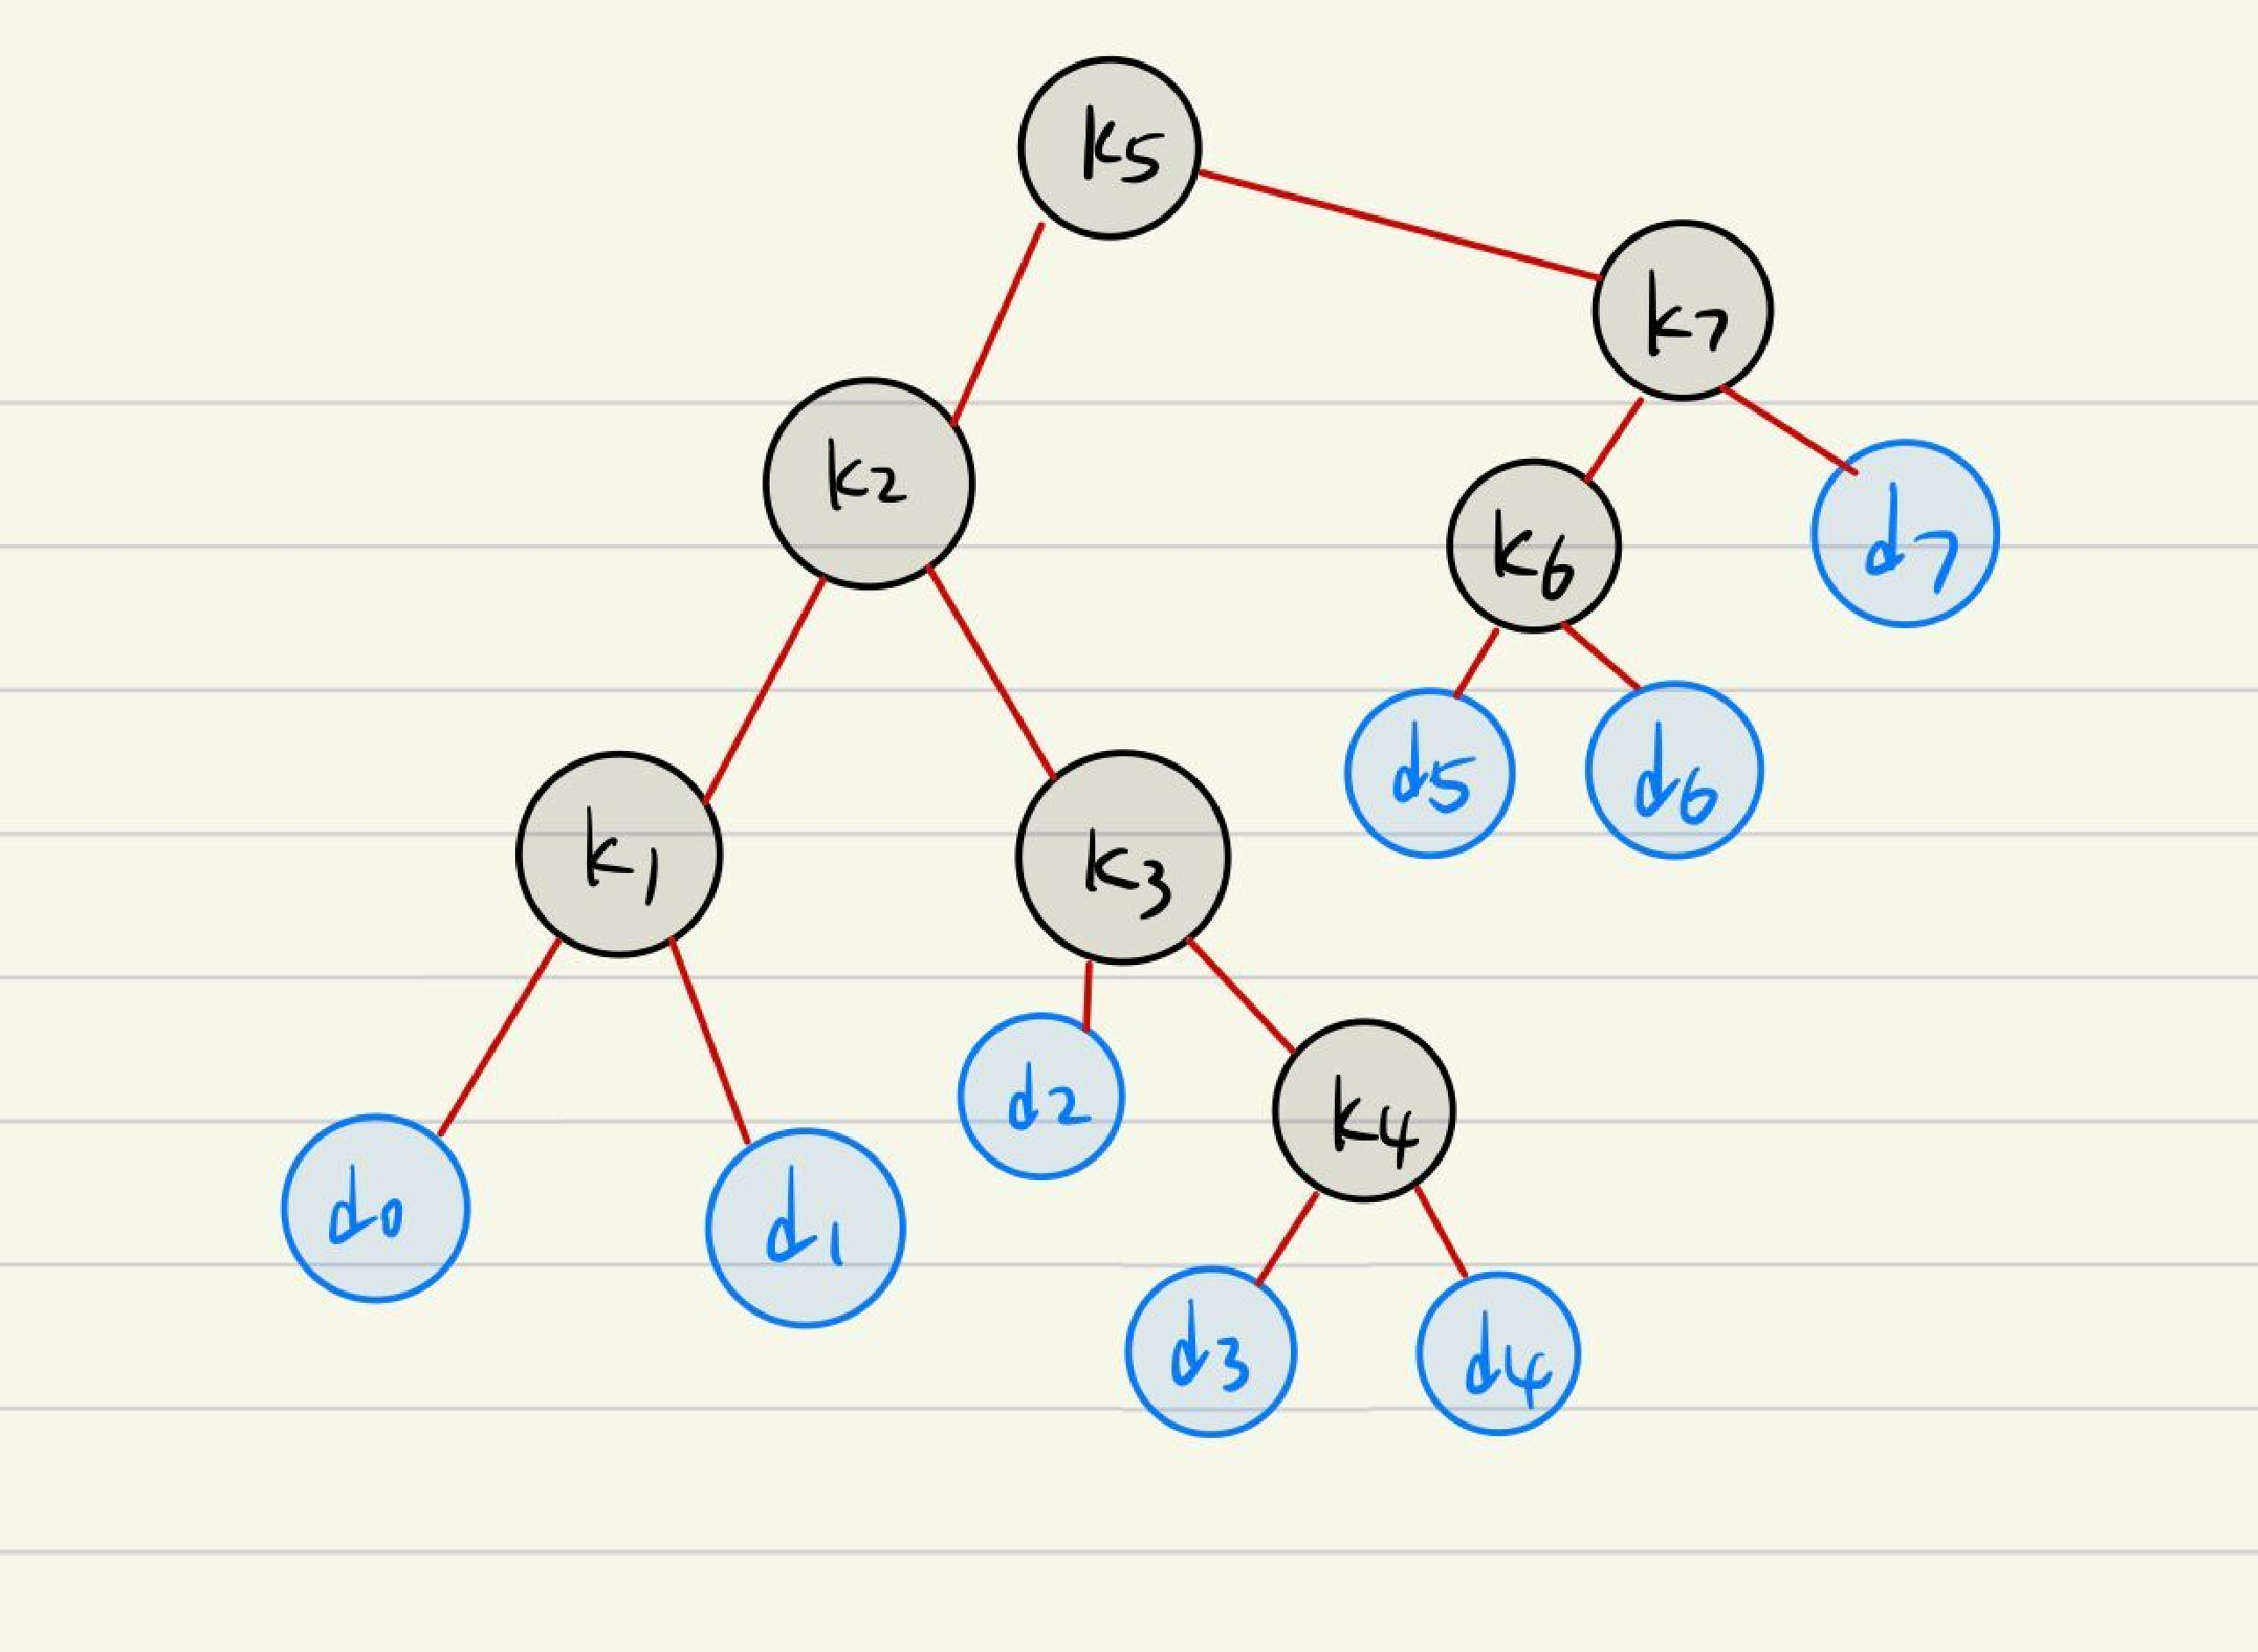
\includegraphics[width=0.5\textwidth]{tree.pdf}
                %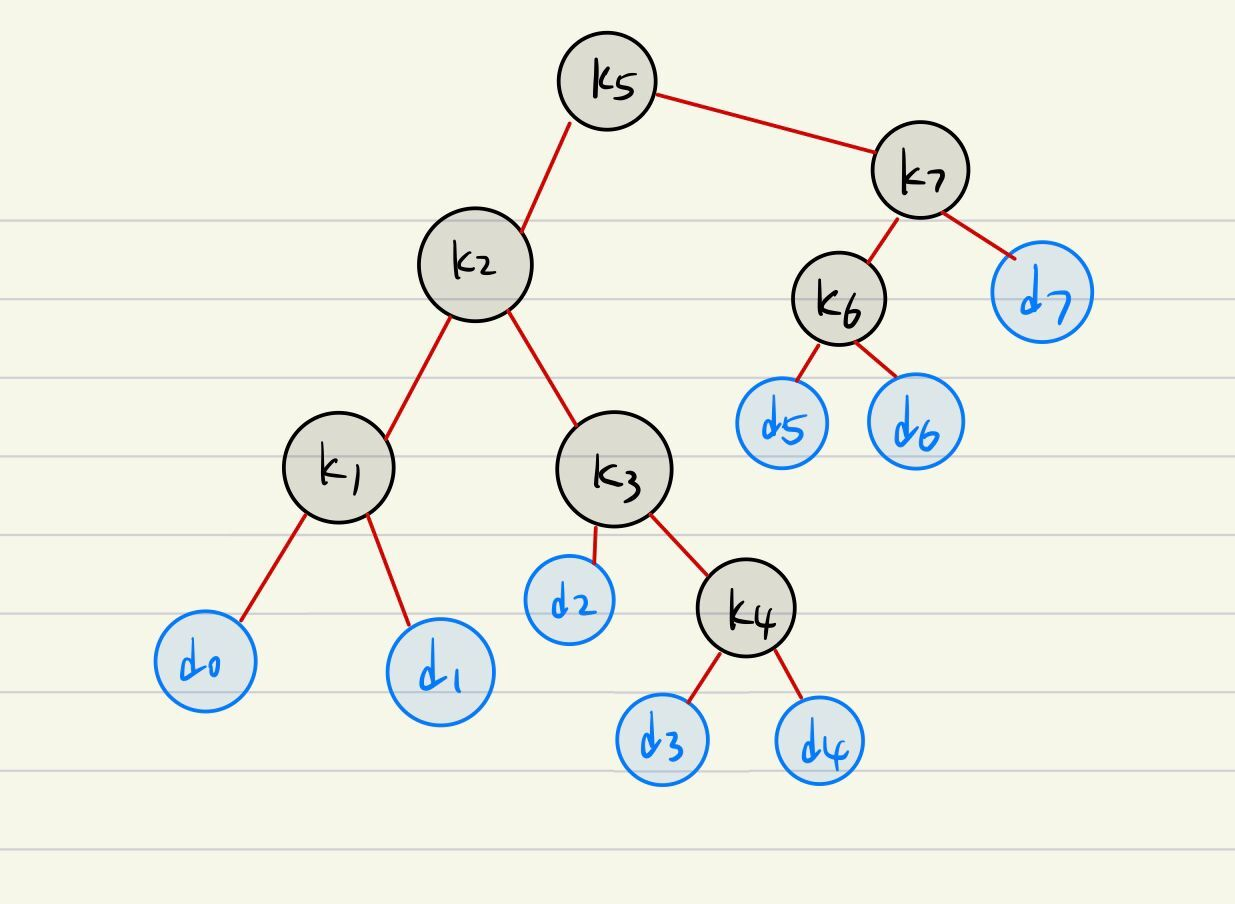
\includegraphics[width=1in]{tree.jpg}
                \caption{tree} %最终文档中希望显示的图片标题
                \label{} %用于文内引用的标签
                \end{figure}
                
                % \begin{figure}[htbp]
                %  \centering
                % 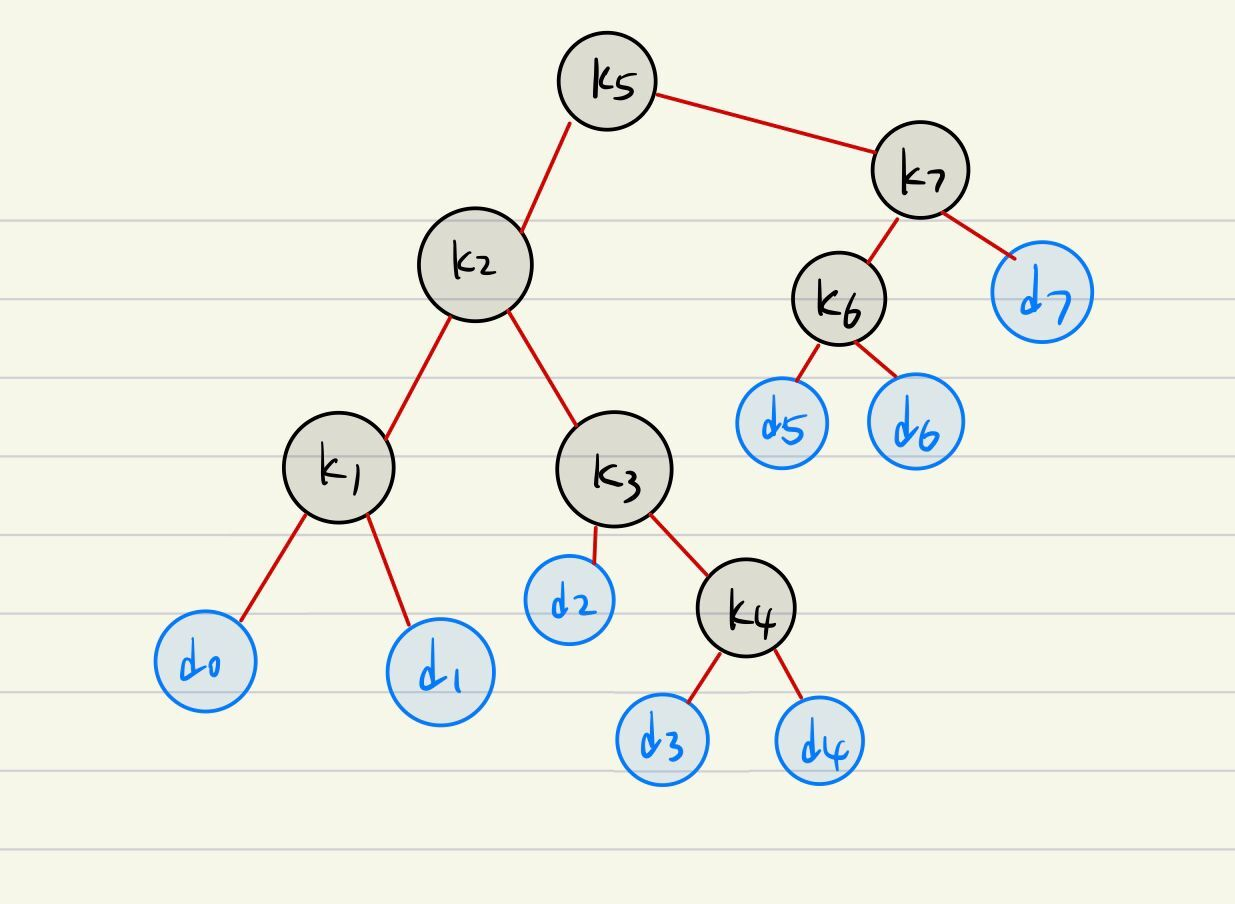
\includegraphics[width=0.8\textwidth]{tree.jpg}
                % \caption{ Tree }
                % \end{figure}
		        
		    \end{solution}
		
		%\newpage
		
		\item \textit{Dynamic Time Warping Distance.} \textbf{DTW} stretches the series along the time axis in a dynamic way over different
		portions to enable more effective matching. Let $D T W(i, j)$ be the optimal distance between the first $i$ and first $j$ elements of two time series $\bar{X}=\left(x_{1} \ldots x_{n}\right)$ and $\bar{Y}=\left(y_{1} \ldots y_{m}\right),$ respectively. Note that the two time series are of lengths $n$ and $m$, which may not be the same. Then, the value of $D T W(i, j)$ is defined recursively as follows:
		$$
		DTW(i, j)=\left|x_{i}- y_{j}\right|+\min(DTW(i, j-1), DTW(i-1, j), DTW(i-1, j-1))
		$$
		
		\begin{enumerate}
			\item Implement the proposed DTW algorithm in C/C++ and analyze the time complexity of your implementation. ({\color{blue}The framework Code-DTW.cpp is attached on the course webpage}). Two test cases have been given in the source code. 
			\item The window constraint imposes a minimum level $w$ of positional alignment between matched elements. The window constraint requires that $DTW(i, j)$ be computed only when $|i-j| \leq w$. Modify your code to add a window constraint and give the results of $ w=0 $ and $ w=1 $ on the two test cases. 
		\end{enumerate}
		    \begin{solution}
		        %Uncomment this block to write your solution.
		        \\(1):\\
		        The code can be found in appendix $2$, and the pictures of results can be found in appendix $3$.
		        \\Here are the time complexity analysis: \\
		        The time complexity of the DTW algorithm is  $O\left(NM\right)$, where $N$ and $M$ are the lengths of the two input sequences. When we assume that $ N\geq M$, the time complexity can be up to  $N^2$. 

		        
		        \\(2):\\
                The code can be found in appendix $2$, and the pictures of results can be found in appendix $3$.
		        
		        
		        
		        
		    \end{solution}
		
	\end{enumerate}
	
	\vspace{20pt}
	
	\textbf{Remark:} You need to include your .pdf and .tex and {\color{red}\emph{$2$}} source code files in your uploaded .rar or .zip file. Screenshots of test case results are acceptable.
	


\newpage

\begin{appendices}
\section{First appendix: Code-OBST.cpp}
\textcolor[rgb]{0.98,0.00,0.00}{\textbf{Input C++ source1:}}
\lstinputlisting[language=c++]{./Code-OBST.cpp}

%\t

%\section{Second appendix}

%\textcolor[rgb]{0.98,0.00,0.00}{\textbf{Input python source2:}}
%\lstinputlisting[language=python]{./code/fire_data.py}

\end{appendices}


\newpage

\begin{appendices}
\section{Second appendix: Code-DTW.cpp}
\textcolor[rgb]{0.98,0.00,0.00}{\textbf{Input C++ source1:}}
\lstinputlisting[language=c++]{./Code-DTW.cpp}

%\t

%\section{Second appendix}

%\textcolor[rgb]{0.98,0.00,0.00}{\textbf{Input python source2:}}
%\lstinputlisting[language=python]{./code/fire_data.py}

\end{appendices}

\newpage

\begin{appendices}
\section{Third appendix: Outcome pictures}

\begin{figure}[H] %H为当前位置,!htb为忽略美学标准,htbp为浮动图形
\centering %图片居中
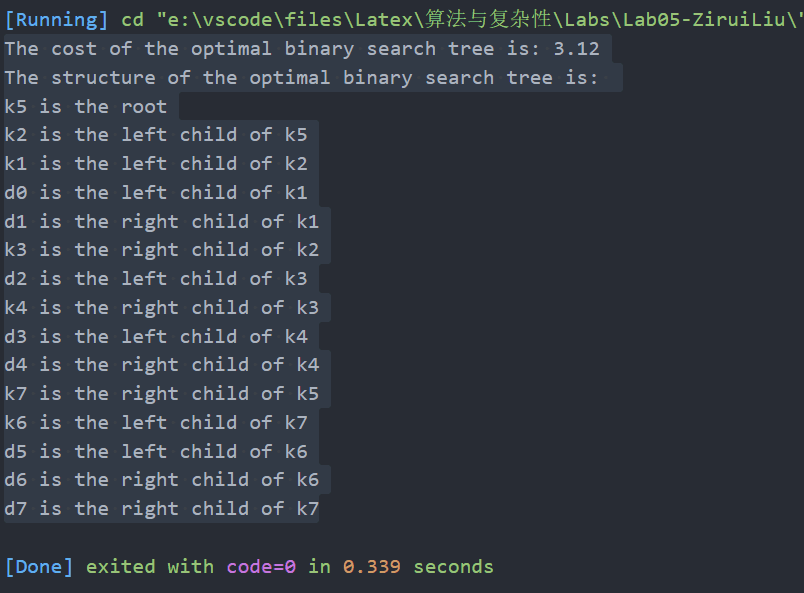
\includegraphics[width=0.7\textwidth]{1.png} %插入图片,[]中设置图片大小,{}中是图片文件名
\caption{OBST} %最终文档中希望显示的图片标题
\label{} %用于文内引用的标签
\end{figure}

\begin{figure}[H] %H为当前位置,!htb为忽略美学标准,htbp为浮动图形
\centering %图片居中
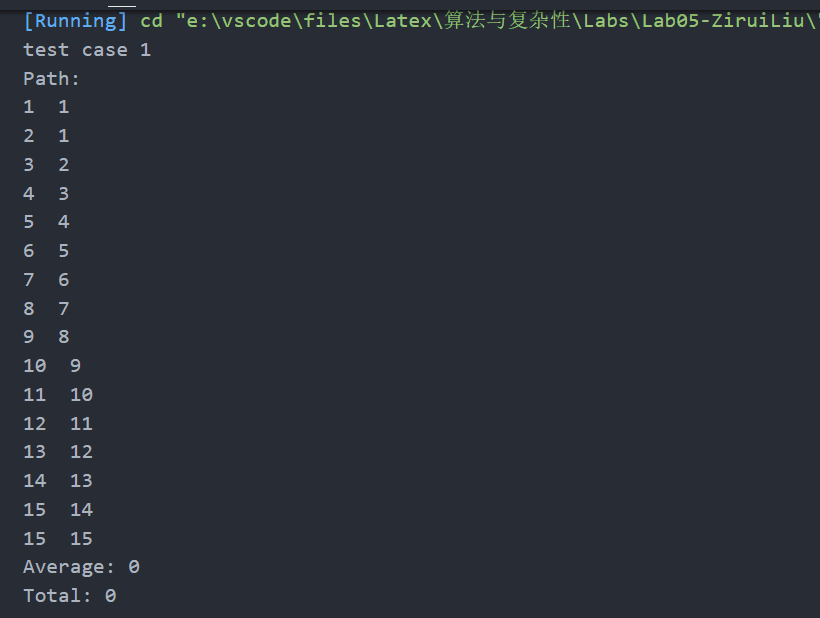
\includegraphics[width=0.7\textwidth]{2.png} %插入图片,[]中设置图片大小,{}中是图片文件名
\caption{DTW1} %最终文档中希望显示的图片标题
\label{} %用于文内引用的标签
\end{figure}

\begin{figure}[H] %H为当前位置,!htb为忽略美学标准,htbp为浮动图形
\centering %图片居中
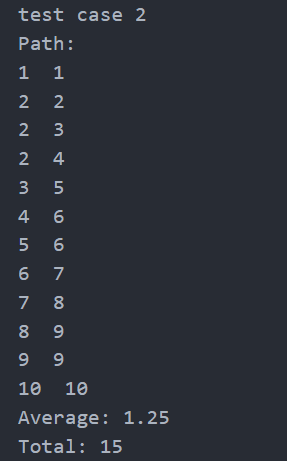
\includegraphics[width=0.7\textwidth]{3.png} %插入图片,[]中设置图片大小,{}中是图片文件名
\caption{DTW2} %最终文档中希望显示的图片标题
\label{} %用于文内引用的标签
\end{figure}

\begin{figure}[H] %H为当前位置,!htb为忽略美学标准,htbp为浮动图形
\centering %图片居中
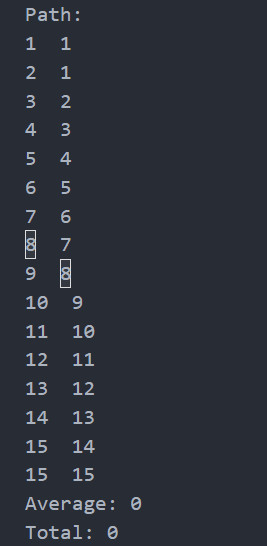
\includegraphics[width=0.7\textwidth]{4.png} %插入图片,[]中设置图片大小,{}中是图片文件名
\caption{DTW3} %最终文档中希望显示的图片标题
\label{} %用于文内引用的标签
\end{figure}

\begin{figure}[H] %H为当前位置,!htb为忽略美学标准,htbp为浮动图形
\centering %图片居中
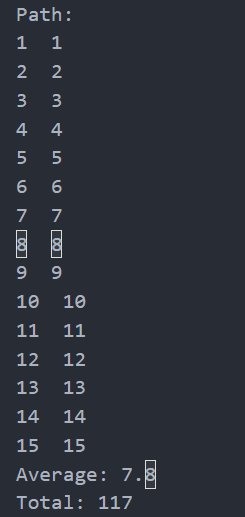
\includegraphics[width=0.7\textwidth]{5.png} %插入图片,[]中设置图片大小,{}中是图片文件名
\caption{DTW4} %最终文档中希望显示的图片标题
\label{} %用于文内引用的标签
\end{figure}

\begin{figure}[H] %H为当前位置,!htb为忽略美学标准,htbp为浮动图形
\centering %图片居中
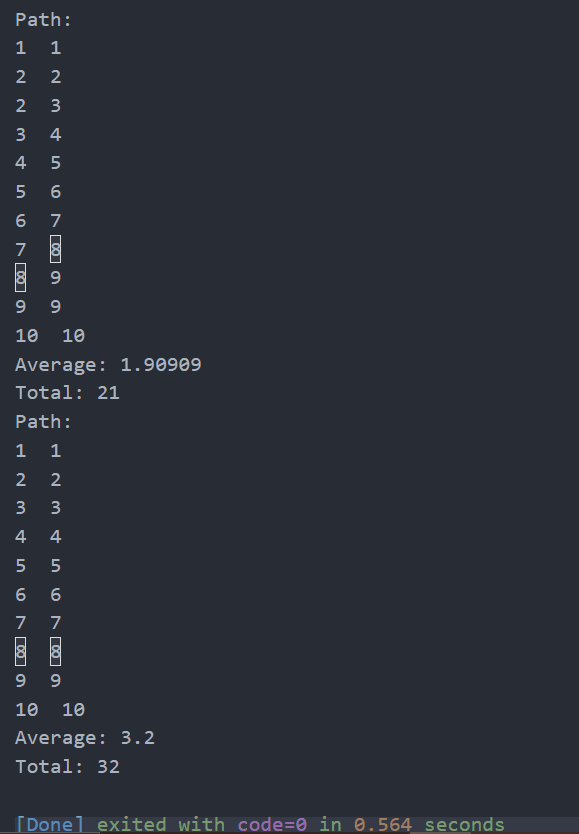
\includegraphics[width=0.7\textwidth]{6.png} %插入图片,[]中设置图片大小,{}中是图片文件名
\caption{DTW5} %最终文档中希望显示的图片标题
\label{} %用于文内引用的标签
\end{figure}


\end{appendices}
	
	%========================================================================
\end{document}
